\documentclass[12pt,a4paper]{report}
\usepackage[utf8]{inputenc}
\usepackage[english]{babel}
\usepackage{amsmath}
\usepackage{amsfonts}
\usepackage{amssymb}
\usepackage{makeidx}
\usepackage{graphicx}
\usepackage{lmodern}
\usepackage{fourier}
\usepackage{graphicx}
\usepackage{subcaption}
\usepackage{setspace}
\usepackage{wrapfig}
\usepackage{lscape}
\usepackage{rotating}
\usepackage{epstopdf}
\usepackage[left=2cm,right=2cm,top=2cm,bottom=2cm]{geometry}
\author{Guillem Bagaria i Portet}
\title{Personality Trait Classifier from Natural Language}

\begin{document}
\doublespacing
\maketitle
\tableofcontents
\singlespacing
\chapter{Initial data exploration}

\section{The data}

\paragraph{About the data:} 

\paragraph{} The used dataset consists of 10,000 transcripts extracted from video clips of people talking directly into the camera. Each transcript has an assigned label for each one one of the 6 labels (extraversion', 'neuroticism', 'agreeableness', 'conscientiousness', 'openness' and 'interview'). The first 5 are from the Big Five personality traits, originally developed in 1961 in a US Air force paper, very commonly cited in psychological literature \cite{bigFive}.
\paragraph{} In order to estimate the ground truth, human perception while seeing the videos was used through Amazon Mechanical Turk \cite{chalearn}. Each rater had to rank a small batch of paired videos by comparing them, and point out which one was more extroverted, neurotic, interviewable, etc. All 10,000 videos were pairwise compared 321,684 times producing, for each label, a ranking between 0 and 1. The values are centered relatively close to 0.5 except for openness and agreeableness which are both centered closer to 0.6.

\paragraph{}  Because the labels are treated as a partial class membership (as opposed to multiple membership, which would imply that only one if them is actually true), in the \emph{ChaLearn LAP 2016} paper they use an accuracy measure as an average distance from the ground truth for each personality trait. The best way to do this is to calculate the performance as some kind of distance from the ground truth value.

\paragraph{} If we instead tried to assess the dominant trait, interpreting the ground truth and predicted labels as a multiple membership problem, it would be necessary to generate a label defined as such: $t=1$ if the highest ranked trait corresponds to the highest ranked trait in the ground truth, $t=0$ otherwise. However, even before trying this, I believe this reduces drastically the amount of data that might otherwise be valuable to for a learning algorithm. Similarly to the case of ranking the "interview" labels and setting an arbitrary threshold.


\begin{sidewaysfigure}
    \centering
    \begin{subfigure}[b]{0.32\textwidth}
        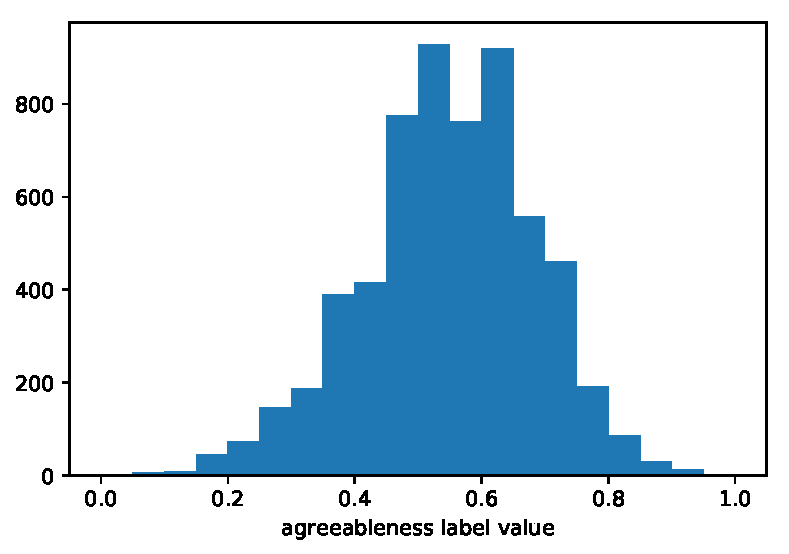
\includegraphics[width=\textwidth]{imgs/agreeableness_label_value.pdf}
        \caption{agreeableness}
        \label{fig:agreeableness}
    \end{subfigure}
    ~ %add desired spacing between images, e. g. ~, \quad, \qquad, \hfill etc. 
      %(or a blank line to force the subfigure onto a new line)
    \begin{subfigure}[b]{0.32\textwidth}
        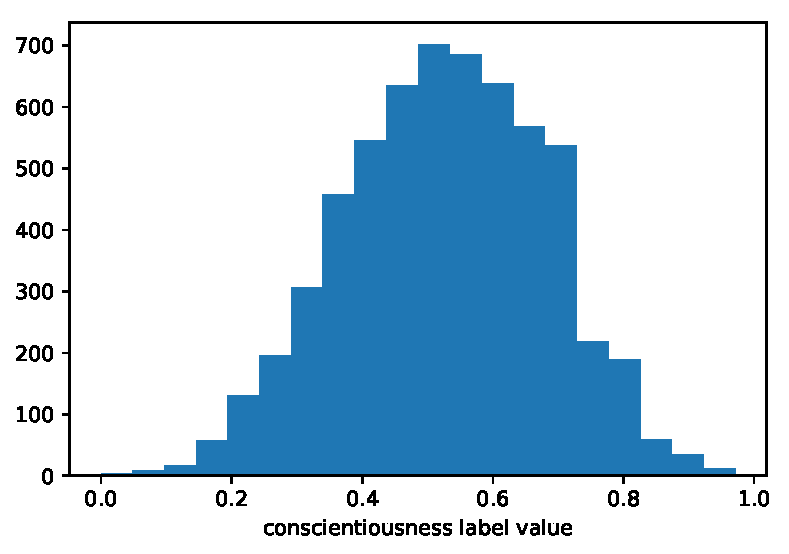
\includegraphics[width=\textwidth]{imgs/conscientiousness_label_value.pdf}
        \caption{conscientiousness}
        \label{fig:conscientiousness}
    \end{subfigure}
    ~ %add desired spacing between images, e. g. ~, \quad, \qquad, \hfill etc. 
    %(or a blank line to force the subfigure onto a new line)
    \begin{subfigure}[b]{0.32\textwidth}
        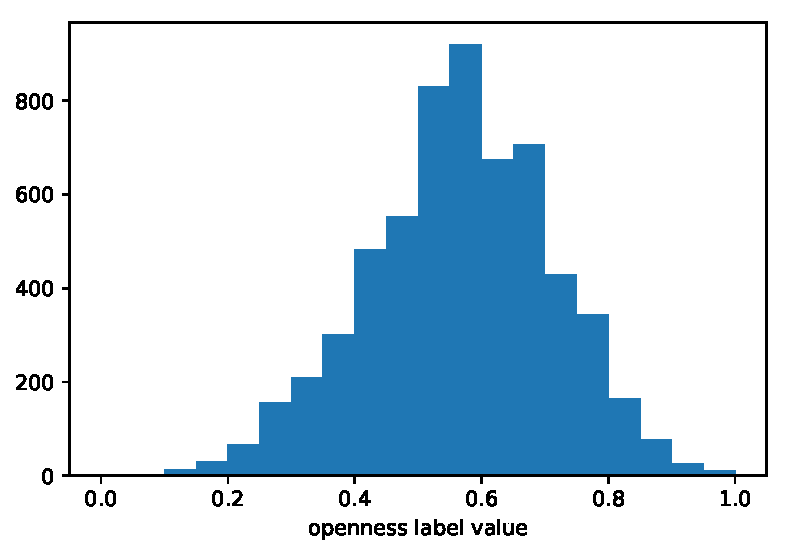
\includegraphics[width=\textwidth]{imgs/openness_label_value.pdf}
        \caption{openness}
        \label{fig:openness}
    \end{subfigure}
    \begin{subfigure}[b]{0.32\textwidth}
        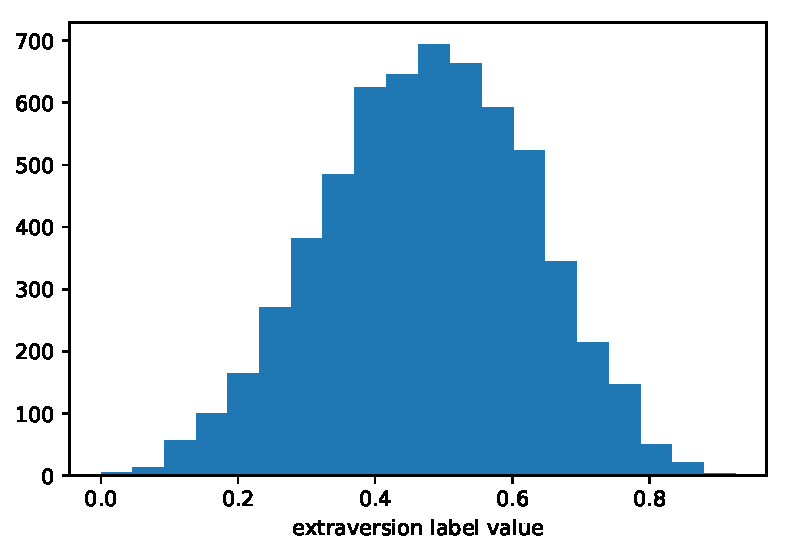
\includegraphics[width=\textwidth]{imgs/extraversion_label_value.pdf}
        \caption{extraversion}
        \label{fig:extraversion}
    \end{subfigure}
        \begin{subfigure}[b]{0.32\textwidth}
        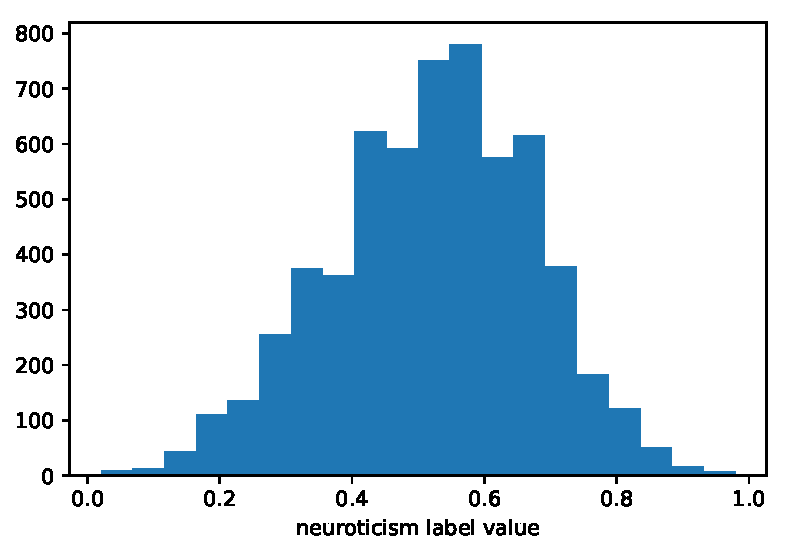
\includegraphics[width=\textwidth]{imgs/neuroticism_label_value.pdf}
        \caption{neuroticism}
        \label{fig:neuroticism}
    \end{subfigure}
    \begin{subfigure}[b]{0.32\textwidth}
        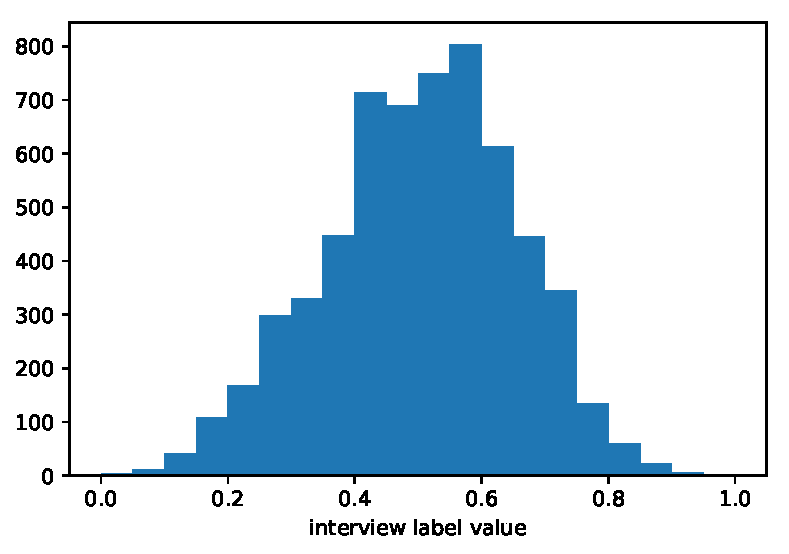
\includegraphics[width=\textwidth]{imgs/interview_label_value.pdf}
        \caption{interview}
        \label{fig:interview}
    \end{subfigure}
    \caption{Distribution of the jobScreening data label values}\label{fig:jobscreeninglabels}
\end{sidewaysfigure}

\paragraph{About the \emph{interview} label:}

\paragraph{}The values for the interview label are 0.504 mean and 0.514 median and range from 0.0 to 1.0, the higher, the more inteviewable that person is. The job in question is not determined, so the labels are given for personality traits reasons. However, this might be a naïve understanding, because there might be significant bias towards other parameters that are not counted in the labels, such as gender or age. Biases should be lower (albeit not nonexistent) when asking for the more "objective" personality traits listed above.

\paragraph{} The way the data is collected suggests that the personality traits are related to the \emph{interview} label value. In order to better understand the predictions I would first use a simple linear regression model to find how the personality traits predict the \emph{interview} label. The expectation is that this will
\begin{enumerate}
\item point out the factors (parameters) that determine interviewability and
\item isolate hypothetical bias in the \emph{interview} label.
\end{enumerate}

\section{Fleiss's kappa coefficient ($\kappa$)} Fleiss's kappa coefficient ($\kappa$), as described in \cite{fleisskappa} is a statistic which measures inter-rater agreement in a many rater scenario, for qualitative (categorical) ratings that takes into account the possibility of agreement occurring by chance. In the case of the labels used in this dataset, we can use this as a threshold to reject labels that are deemed inconclusive. This fact adds to the problem of low contrast labels for the classifier algorithm during the training.

\paragraph{}This coefficient can be calculated as $$\kappa = \frac{p_0-p_e}{1-p_e}$$ where $p_0$ is the accuracy among raters, and $p_e$ is the hypothetical probability of agreeing by chance, calculated as $$p_e=  \sum_{j=1}^k p_{j}^2$$ whith $$p_j = \frac{1}{N^2}\sum_{i=1}^N n_{ij}$$ where $N$ is the total number of raters, $n$ the number of ratings per rater such that $n_{ij}$ and $k$ the number of categories, in this case $k=2$.

\paragraph{} If all raters agree, $\kappa=1$; if there is no agreement, aside from that occurring by chance, $\kappa=0$; if there is less agreement than what would occur by chance, $\kappa<0$.

\paragraph{} We do not have the data from the ground truth estimation, however it is a reasonable hypothesis that the ambiguous values (close to the mean) are caused by higher disagreement between raters, as described by the Bradley–Terry model \cite{bradleyterry}, used in the ranking of the clips.

%\section{EmotiW dataset}
%
%\paragraph{} This dataset consists of 1154 video documents no more than a few seconds long, extracted from movies. Each document is labelled in a separate \emph{.xml} document as such: \emph{Movie Title, Start Time of the clip in the film, the Length of the clip, Age of the actor, Age of the character, Gender, Name of the actor and Pose.}
%
%\paragraph{} The clips are placed in folders named after their corresponding emotion label: \emph{Angry, Disgust, Happy, Neutral, Sad, Fear or Surprise}.


\section{Interview label prediction}

\paragraph{} The analysis and information extraction of the transcripts is the first step. In order to do this the Job Screening data is used to create a binary classifier using the automatic transcripts as data. This algorithm will load the natural language transcript data, divide the data into tokens (one or several words), remove unwanted tokens and other unnecessary characters, convert it into a TFIDF matrix in order to extract the relevant words. This will later improve the performance of the classifier algorithm.

\paragraph{} The used algorithms to be compared will be a Support Vector Classifier with radial kernel and a Naive Bayes Classifier.

\section{Threshold for dichotomic labels}

\paragraph{} In order to train a classifier model, categorical labels are required. As previously seen, the \emph{interview} label follows a bell curve distribution between 0 and 1. The objective is to dichotomize the label into two categories (0 and 1) in order to feed the Support Vector Classifier.

\paragraph{} Since many documents have a somewhat ambiguous label (that is, close to the mean label value, or $\textasciitilde 0.5$), the threshold for the training process will be centered in order to provide the classifier algorithm with better contrast. The center is set on the median value in order to correct for label imbalances in the initial threshold ranges.

\paragraph{} In order to maximize the the classifier performance it's necessary to find the optimal standard deviation distance away from the mean as the threshold to discard from the training and test sets. Initially, the same standard deviation from the median value from both train and test data was discarded. However, a second experiment was conducted with several fixed values for the test set. In Figure~\ref{fig:Sigma ROC Sigma} are the results for the first case, with identical thresholds applied to both testing an training data. The reasons to do this are not exclusively to make the classifier's job easier, but also to filter out disagreements from the raters, as discussed in the previous section.

\paragraph{} In Figure~\ref{fig:Sigma ROC Sigma}, the standard deviation value as discard threshold of both train \emph{and} test that maximizes the ROC Score. The maximum is found at around Sigma $= 1.72$. The posterior results are decreasing until they start behaving erratically due to small test dataset and overfitting due to the small training set. However, the steady increase in performance is caused both by the increased contrast between labeled documents as well as the decrease in testing sample.

\begin{figure}[b]
        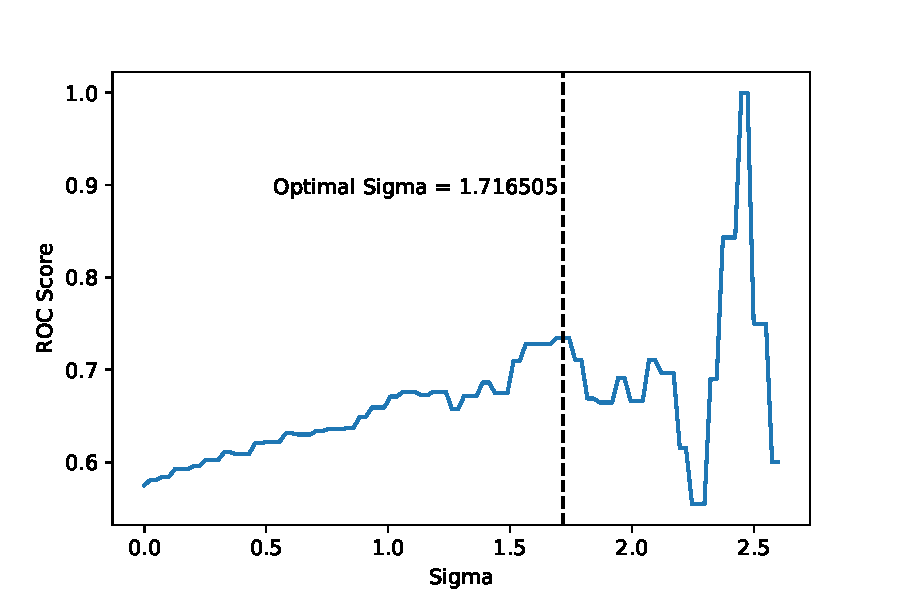
\includegraphics[width=\textwidth]{imgs/Sigma_figure.pdf}
        \caption{Optimal sigma for thresholds applied at both train and test splits.}
        \label{fig:Sigma ROC Sigma}
    \end{figure}

\paragraph{} From the initial results, the following step was to perform the same tests with fixed testing sets. In order to find the optimal test set threshold, several cuts from the test set will be made and subsequently a training set threshold sweep will be calculated for each one. Since decreasing the testing set size directly translates into an improved score, what will be observed is the average slope of the training set sweep. The results can be seen in Figure~\ref{fig:thresholddeletion} and Figure~\ref{fig:testingthresholds}.

\begin{figure}
    \centering
    \begin{subfigure}[b]{0.32\textwidth}
        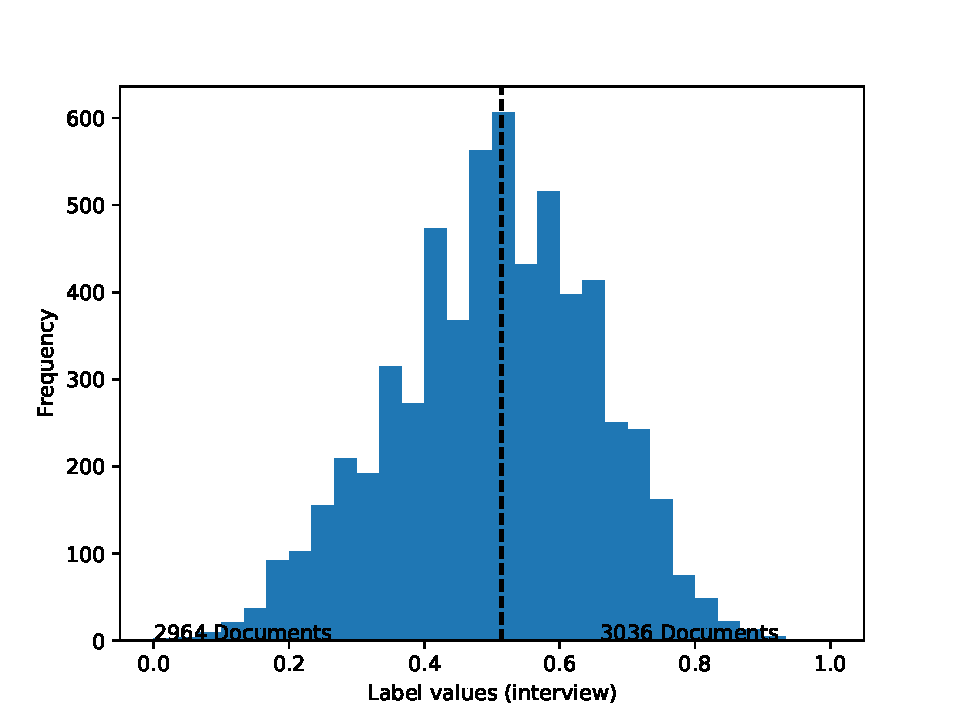
\includegraphics[width=\textwidth]{imgs/training_histogram/0000000_training_histogram.pdf}
        \caption{0 sigma}
        \label{fig:0 sigma}
    \end{subfigure}
    ~ %add desired spacing between images, e. g. ~, \quad, \qquad, \hfill etc. 
      %(or a blank line to force the subfigure onto a new line)
    \begin{subfigure}[b]{0.32\textwidth}
        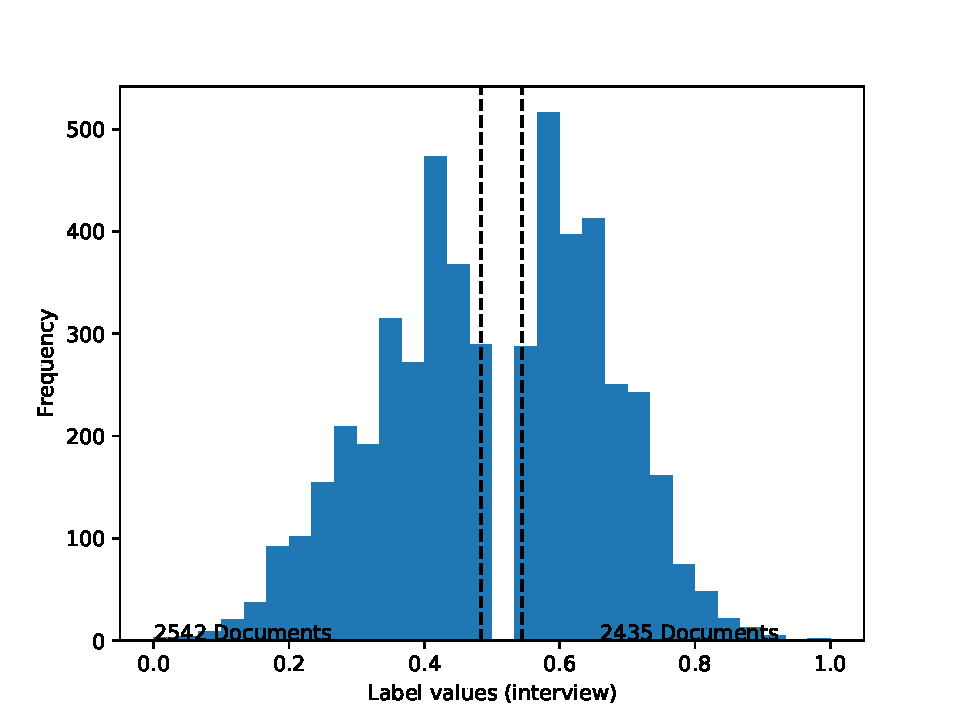
\includegraphics[width=\textwidth]{imgs/training_histogram/0201942_training_histogram.pdf}
        \caption{0.202 sigma}
        \label{fig:0.202 sigma}
    \end{subfigure}
    ~ %add desired spacing between images, e. g. ~, \quad, \qquad, \hfill etc. 
    %(or a blank line to force the subfigure onto a new line)
    \begin{subfigure}[b]{0.32\textwidth}
        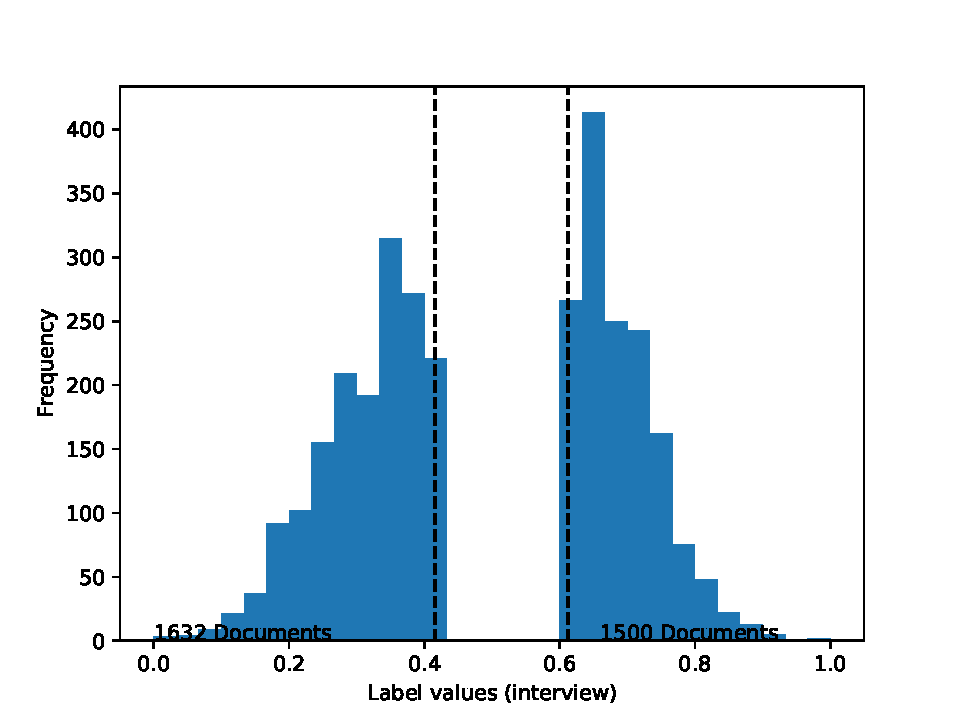
\includegraphics[width=\textwidth]{imgs/training_histogram/0656311_training_histogram.pdf}
        \caption{0.656 sigma}
        \label{fig:0.656 sigma}
    \end{subfigure}
    \caption{Distribution of the jobScreening interview label values after removing increasingly wide central values.}\label{fig:thresholddeletion}
\end{figure}

\paragraph{} The ROC score against the training sigma threshold for each value of removed sigma in the test set can be seen in Figure\ref{fig:testingthresholds} The training set optimal sigma is very stable, at around 0.278. The rate at which the ROC score decreases with training sigma is steeper as the test sigma increases until it reaches 1 sigma. At this point the increase in training sigma has little impact on the ROC suggesting that the dominant factor in the ROC score becomes the small test sample size. The optimal value for which the SVC classifier obtains the best results, given the training and test data are a testing threshold of 0.8 sigma and a training threshold of 0.278 sigma.

\begin{figure}
    \centering
    \begin{subfigure}[b]{0.49\textwidth}
        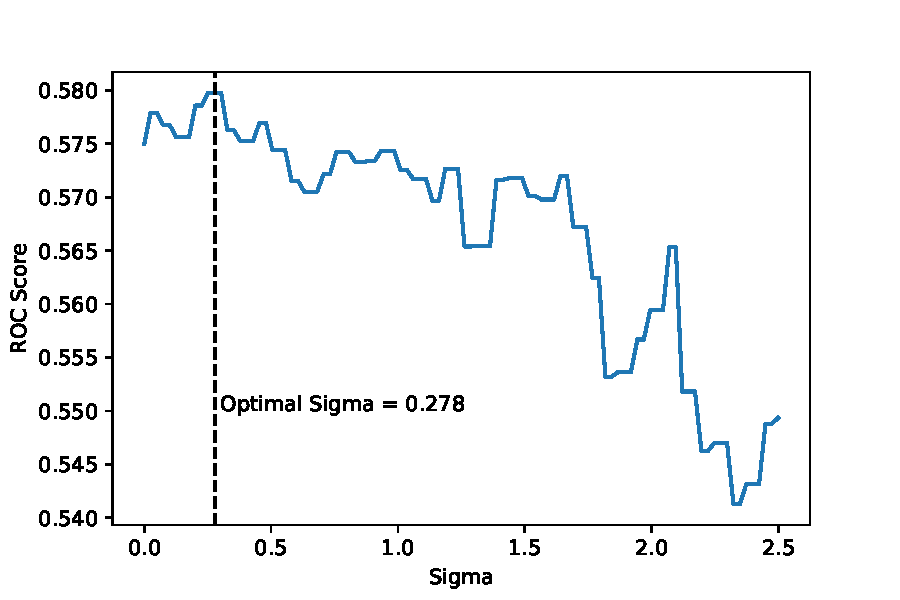
\includegraphics[width=\textwidth]{imgs/180531_Sigma_fixed_test_00.pdf}
        \caption{Complete test set. The score varies very little as the training sigma increases because the test set includes too many ambiguous documents.}
        \label{fig:}
    \end{subfigure}
    ~ %add desired spacing between images, e. g. ~, \quad, \qquad, \hfill etc. 
      %(or a blank line to force the subfigure onto a new line)
    \begin{subfigure}[b]{0.49\textwidth}
        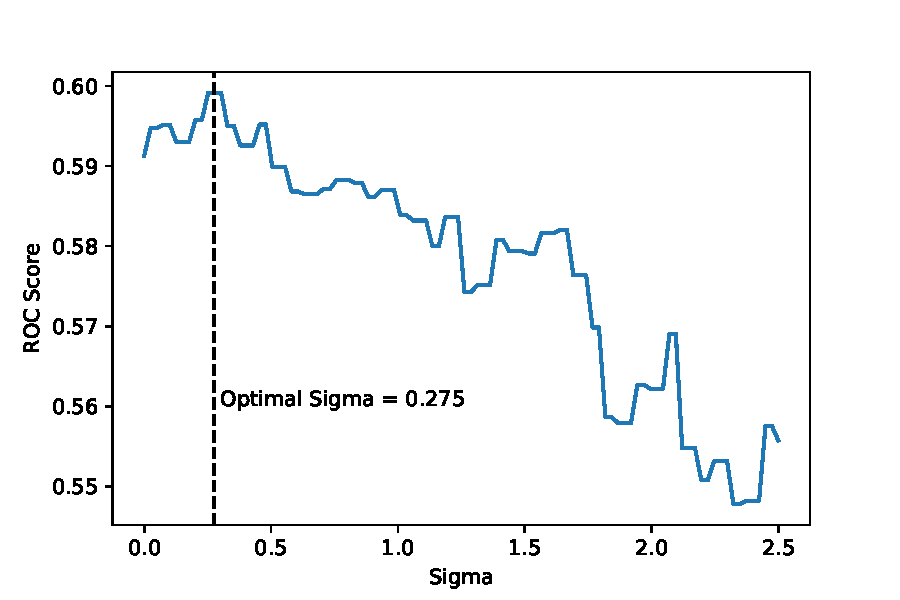
\includegraphics[width=\textwidth]{imgs/180531_Sigma_fixed_test_02.pdf}
        \caption{Test set without 0.2 Sigma. The slope to and from the optimal are steep.\linebreak }
        \label{fig:}
    \end{subfigure}
    ~ %add desired spacing between images, e. g. ~, \quad, \qquad, \hfill etc. 
    %(or a blank line to force the subfigure onto a new line)
    \begin{subfigure}[b]{0.49\textwidth}
        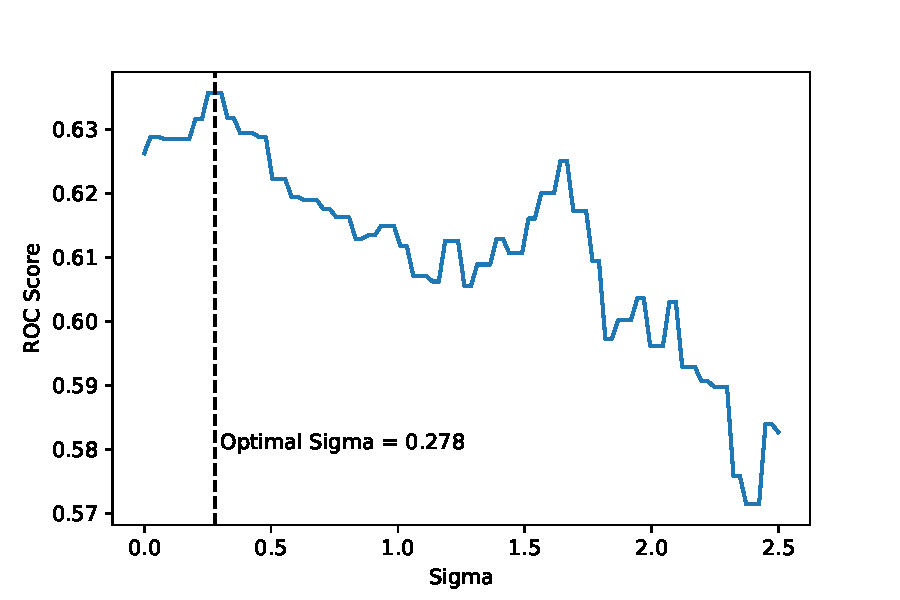
\includegraphics[width=\textwidth]{imgs/180531_Sigma_fixed_test_05.pdf}
        \caption{Test set without 0.5 Sigma. This case shows a steep slope after the optimum.}
        \label{fig:}
    \end{subfigure}
    \begin{subfigure}[b]{0.49\textwidth}
        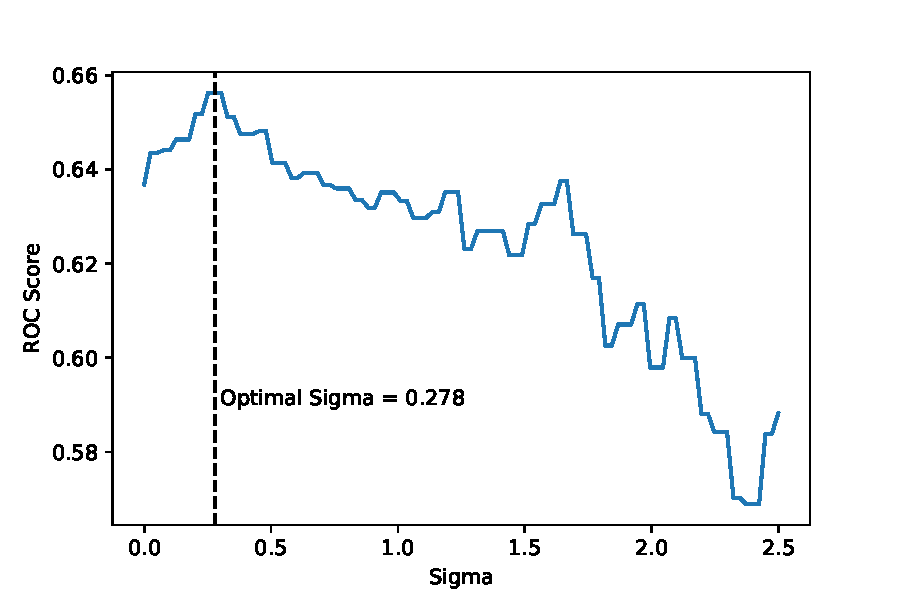
\includegraphics[width=\textwidth]{imgs/180531_Sigma_fixed_test_08.pdf}
        \caption{Test set without 0.8 Sigma. This case shows a steep slope both after and before the optimum.}
        \label{fig:}
    \end{subfigure}
        \begin{subfigure}[b]{0.49\textwidth}
        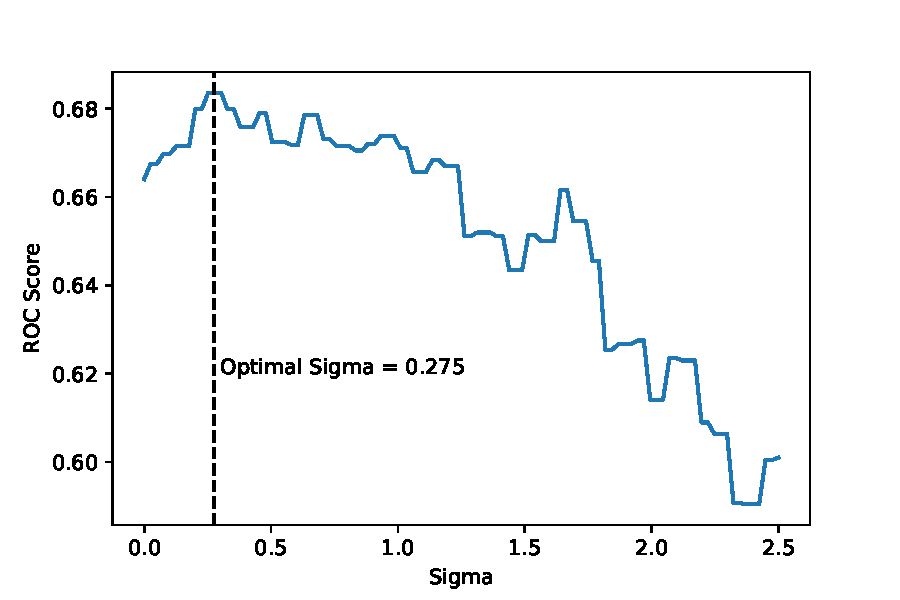
\includegraphics[width=\textwidth]{imgs/180531_Sigma_fixed_test_10.pdf}
        \caption{Test set without 1.0 Sigma. The score plateaus although the training optimal is still consistent with all previous test sets.}
        \label{fig:}
    \end{subfigure}
    \begin{subfigure}[b]{0.49\textwidth}
        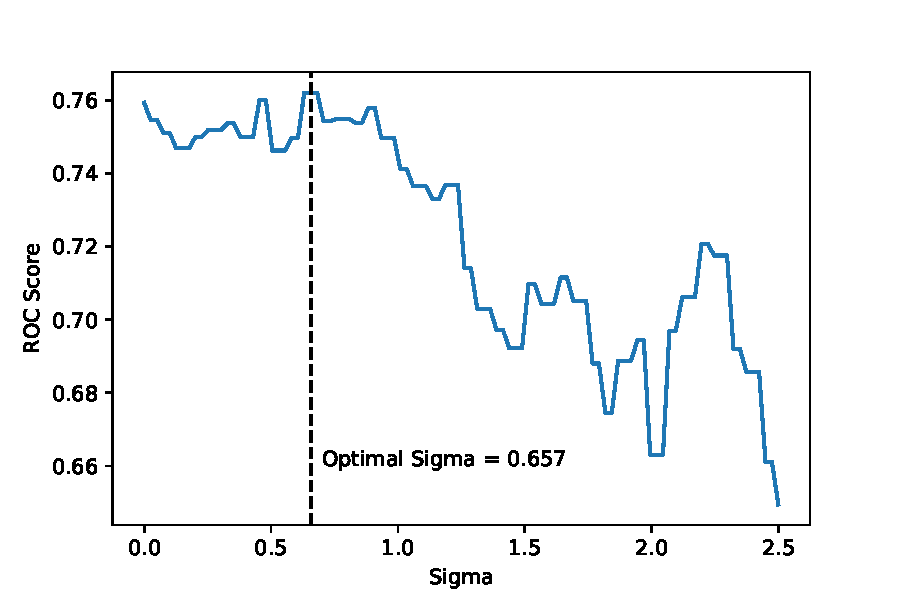
\includegraphics[width=\textwidth]{imgs/180531_Sigma_fixed_test_15.pdf}
        \caption{Test set without 1.5 Sigma. The score shows the same plateau shape, but behaves increasingly erratically, first signs of small test set.}
        \label{fig:}
    \end{subfigure}
    \caption{}
    \label{fig:testingthresholds}
\end{figure}


\paragraph{} The plots can be seen in Figure~\ref{fig:OptimalSigmaFixedTestSVC} for the Support Vector Classifier and in Figure~\ref{fig:OptimalSigmaFixedTestNB} for the Naive Bayes Multinomial classifier.

\begin{figure}[b]
        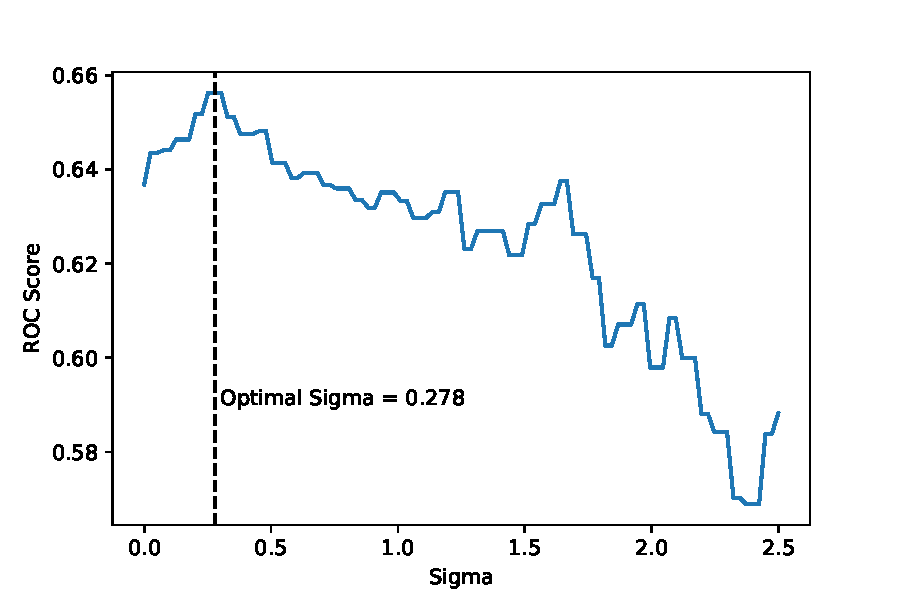
\includegraphics[width=\textwidth]{imgs/180531_Sigma_fixed_test_08.pdf}
        \caption{rbf kernel SVC}
        \label{fig:OptimalSigmaFixedTestSVC}
\end{figure}

\begin{figure}[b]
        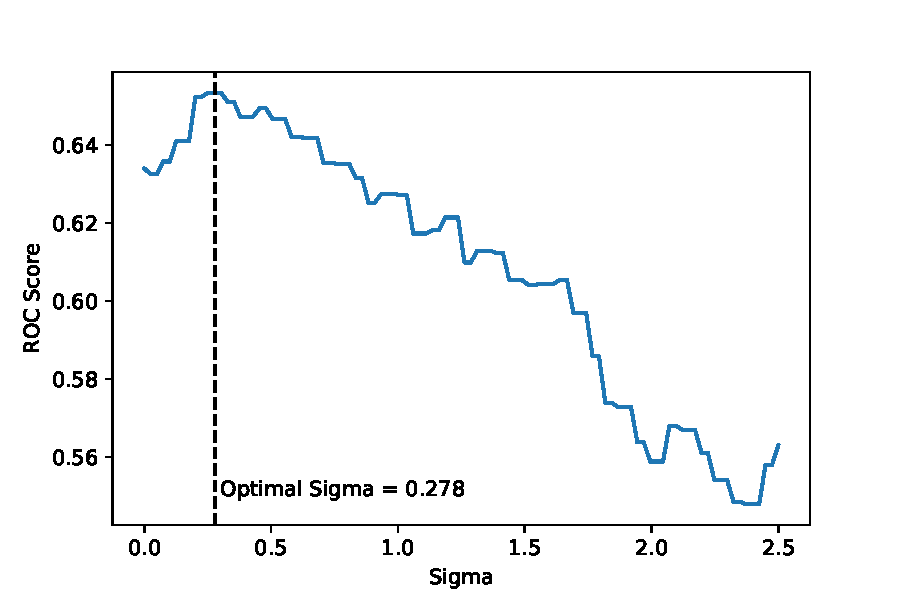
\includegraphics[width=\textwidth]{imgs/180601_ROC_NBayes_00.pdf}
        \caption{Naive Bayes Mutinomial classifier}
        \label{fig:OptimalSigmaFixedTestNB}
\end{figure}

\paragraph{} The sigma parameters together with a Naive Bayes Multinomial classifier produce a stable optimal value, but the ROC score decreases some decimal points compared to an rbf kernel SVC.

\chapter{Natural language processing}
\section{Text normalization}
\paragraph{} The first stage in the implementation is to perform the normalization of the data, in this case the text.

\paragraph{} Numbers are substituted by a flag term. In the data numbers occur when the transcript is unavailable due to unintelligibility.

\paragraph{} All words are converted to lowercase in order to homogenize.


\section{Term Frequency - Inverse Document Frequency} The text data is treated as a Bag of Words. Each document is encoded in a matrix where each column corresponds to one of the words that it contains. After this is done for all documents, the count is divided by the number of occurrences of that word in all documents, so as to obtain a relative importance of each word. Thus the words that are common will have a lower weighting than words that are rare.

\paragraph{} By doing this we are assuming that the rare words are more significant than the others in the classification algorithm. Under this assumption, this is a feature extraction process.

\paragraph{} After several tests, the results were not significantly improved by using n-grams larger than 1. This makes the matrix around 13,000 columns wide, which correspond to each one of the different words.

\section{Model selection} In order to find the appropriate model for the classifier the most obvious was using a Support Vector Classifier. Support Vector Machines in general perform very well in high.

\paragraph{} As a baseline to compare with, a multinomial Naive Bayes classifier was used. This was chosen because of its simplicity, especially in the Grid Search algorithm, as it has only one intrinsic parameter to optimize.

\paragraph{} Aside from this, as is the case with high dimensionality a Generalized Linear Model with Ridge Regression was used \cite{scikit-learn1}. 

\paragraph{} Finally, some test were conducted with a Random Forest classifier in order to test out the computation costs of the Gris Search. A Random Forest contains many parameters that can be tuned, e.g. the number of trees, the depth of the trees, the threshold for the number of samples required to split a node or a leaf and bootstrapping.

\paragraph{} Of course, this increases the computation cost exponentially.

\section{Scoring techniques} In assessing the performance of the models, several scoring techniques were used.

\begin{list}{•}{}
\item \textbf{Area Under the Receiver Operating Characteristic Curve} obtained by plotting the True Positive Rate against the False Positive Rate. The output value is the area under the curve.
\item \textbf{Accuracy} represents the correct labeling, calculated as $1/(\text{Total population})\cdot (\text{true positive} + \text{true negative})$.
\item \textbf{Precision} or Positive Predictive Value are the correct positive predictions related to all positive predictions, calculated as $$P=(\text{true positive})/(\text{true positive}+\text{false positive})$$
\item \textbf{Recall} are the correct instances of all positive predictions, calculated as 
$$R=(\text{true positive})/(\text{true positive}+\text{false negative})$$
\item \textbf{F1 score} as the harmonic mean of Precision and Recall $$F1=\frac{2}{\frac{1}{\text{Precision}}+\frac{1}{\text{Recall}}}$$
\end{list}

As well as these indicators, Confusion Matrices have also been used in order to assess if the class imbalances were causing all predictions to be single class during the initial test stages.


\chapter{Experimental methodology}

\section{Crossvalidation}

\paragraph{} The results so far are found relying on the data from the given train/test split (4000/2000). K-fold cross-validation on the training and testing sets is performed in order to provide a more solid result and to avoid overfitting. The number of folds will depend inversely on the number of parameters in the model.

\paragraph{} In this case a 3-fold crossvalidation is conducted. This relatively low number was decided based on the requirement of having large enough data to highlight the relevant parameters in each fold.

\paragraph{} In order for the data to remain balanced, the folds are stratified keeping the same proportion of labels than in the original data. This is done to reduce the negative effect of class imbalance. However, we are assuming that the data is independent identically distributed.

\paragraph{} The resulting model will be an average of each one of the models generated in each fold.

\section{Parameter Grid-Search}

\paragraph{} A fine tuning of the algorithm's parameters is required, as an implementation of the study done in the previous sections. A Grid-Search algorithm is implemented to establish the values of the parameters of each tested model. For example, the $\gamma$ and $C$ for the Support Vector Classifier, $\alpha$ in the case of a Naive Bayes multinomial classifier, or n estimators, max features, max depth, min samples split, min samples leaf and bootstrap in the case of a Random Forest classifier, which can be either numeric or logical.

\paragraph{} Grid-Search cannot be performed normally on a cross-validation setting. If the parameters are tuned using Grid-Search and then the model is trained with the optimal given parameters, the accuracy results would be artificially inflated. That is why the parameters will be crossvalidated on the trainig set, evaluated using the test set. The model will be then trained again using the train and test sets using crossvalidation and scored using the previously unseen  validation set for which the ground truth is also available.

\section{Weighting the labels}
\paragraph{} As seen in the previous section, the documents with ambiguous labels are problematic for training, but removing them altogether poses other problems we have already seen and decreases the data size. To address this, an alternative method was devised.

\paragraph{} The labels that are further from the mean value are expected to be more valuable for the classifier model because they are more likely to contain features with higher contrast. In order to feed this knowledge to the model, a weight is matched to each label proportional to its value. There are two functions that have been used; a parabolic function and a complementary Normal distribution.

\paragraph{} The parabola is defined as having values $y=1$ both when label values are $x=0$ and $x=1$, while having the vertex aligned with the median of the labels values $x=$median. The only free parameter of the parabola is the minimum weight, i.e., what will the $y$ value be when $x=$median. This is used as a model hyper-parameter and is optimized together with the intrinsic parameters of each model.
$$y=ax^2+bx+c$$

By imposing said conditions, $c=1$, $b=-a$ and $a=\frac{w-1}{m^2-m}$, where $w$ is the vertex of the parabola or minimum weight and $m$ is the mean of the label values.

\paragraph{} The complementary to a Normal distribution is calculated in a similar way. First, a standard normal distribution is fit to the label values as follows:

$$y=\frac{1}{\sqrt{2\pi s^2}}e^{-\frac{(x-m)^2}{2s^2}}$$

where $m$ is again the mean and $s$ is the standard deviation of the label values. Then, a normalization process is applied to the list of $y$ values:

$$y_\text{normalized} = 1-\frac{y}{\max(y)}(1-w) $$

This scales the weight values inside the $[0,1]$ interval and incorporates the $w$ minimum weight, as in the parabola function, to be optimized as a hyper-parameter of the model. This factor is then subtracted from 1 in order to obtain the complimentary values.

\begin{figure}
    \centering
        \begin{subfigure}[b]{0.45\textwidth}
        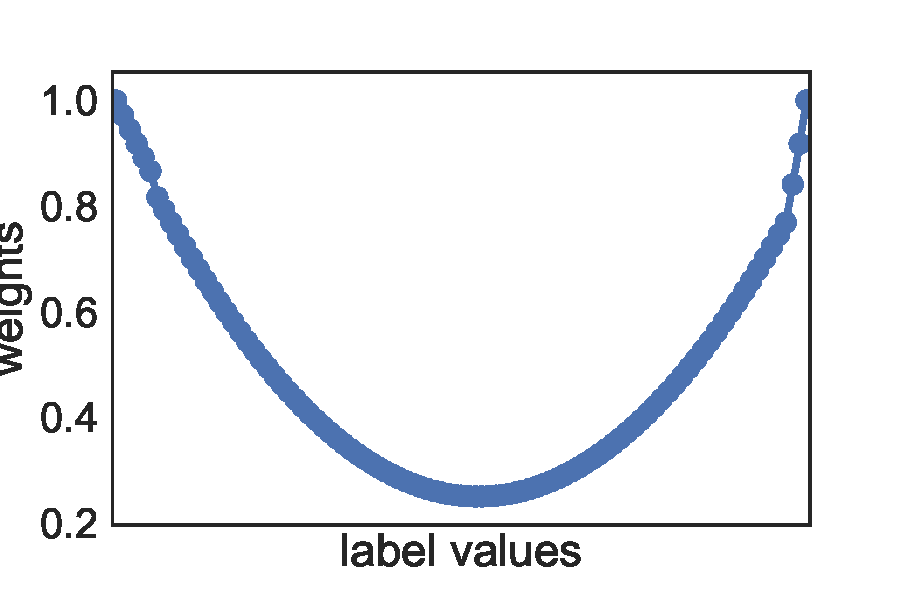
\includegraphics[width=\textwidth]{imgs/180630_ParabolicWeighting_example.pdf}
        \caption{Calculated weights vs label values using a parabolic function, with the minimum weight optimized at 0.25.}
        \label{fig:complementary_Normal_weights}
    \end{subfigure}
    \begin{subfigure}[b]{0.45\textwidth}
        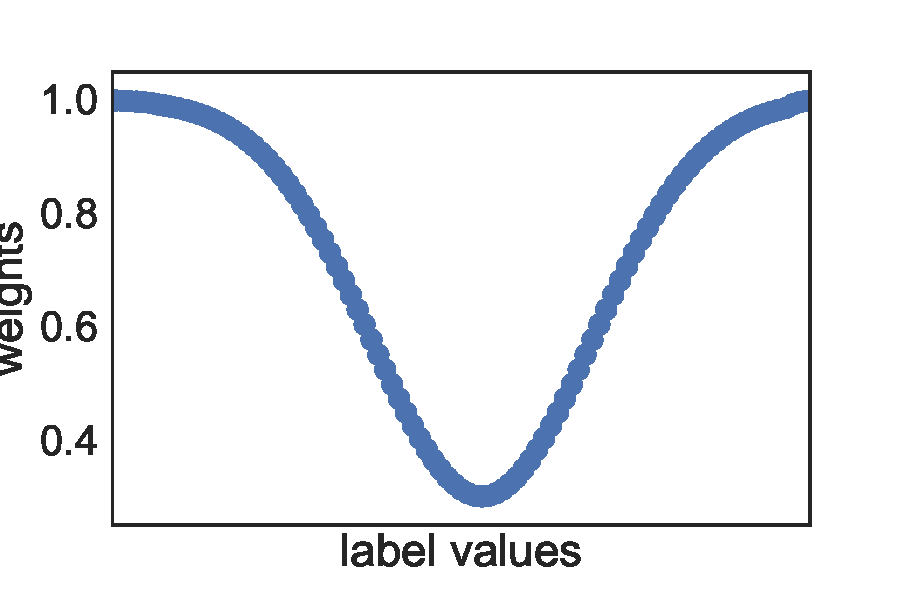
\includegraphics[width=\textwidth]{imgs/180628_1NormalWeighting_example.pdf}
        \caption{Calculated weights vs label values using the complementary to a Normal distribution, with the minimum weight optimized at 0.3.}
        \label{fig:parabolic_weights}
    \end{subfigure}
    \caption{}
    \label{fig:all_weights}
\end{figure}


\paragraph{} In Table~\ref{tab:scores_weighting_RR_functions} and Table~\ref{tab:scores_weighting_NB_functions} the results for the weighting of the labels modifies the F score.

\section{Principal Components Analysis} 
\paragraph{} The tokenized TFIDF matrix of 1-grams is about 13,000 columns wide. This means that there are 13,000 different words that are used as features for classification (Note that this is without lematization).

\paragraph{} In order to reduce dimensionality of this matrix, improve the computation time and  extract more valuable features, a Principal Components Analysis method is applied  to the matrix (as seen in \cite{call_satisfaction}), which in the case of text can also be referred to Latent Semantic Analysis. As its name suggests, the intention behind this is highlighting the latent structure in the combinations of words that might determine the labeling accurately.

\paragraph{} This is in fact a Truncated Singular Value Decomposition that effectively projects the large matrix into a smaller space of a given size. This performs a dimensionality reduction by means of Truncated Singular Value Decomposition. Contrary to PCA, this estimator does not center the data before computing the SVD, so it can work with sparse matrix data types more efficiently \cite{scikit-learn1}.

\paragraph{} The size of the transformed space is arbitrary but of course can greatly affect the performance of the model later on. As reference, the space is reduced to a useful size when it is around the square root of the original. In this case, ~13,000 columns will be projected onto just 114.


\chapter{Conclusion and further steps}

\section{Comparative Results}

\paragraph{Data normalization} Table~\ref{tab:scores_text_normalization}, 

\begin{list}{•}{}
\item the highest performance is attained when keeping the stopwords
\item the flagging of numbers and punctuation does not affect the result significantly, and in labels other than \emph{interview} it further confuses the results.
\item for larger n-gram combinations, the results are not improved significantly either.
\end{list} 

\begin{table}[]
\begin{tabular}{rccc}
\multicolumn{1}{l}{} & With Stopwords & \begin{tabular}[c]{@{}c@{}}Normalized and flagged text\\ With stopwords\end{tabular} & \begin{tabular}[c]{@{}c@{}}Normalized and flagged text\\ Without stopwords\end{tabular} \\ \hline
extraversion         & 0.611293       & 0.598147                    & 0.580981                                                                                \\
neuroticism          & 0.628616       & 0.622925                    & 0.608092                                                                                \\
agreeableness        & 0.625293       & 0.634446                    & 0.6221                                                                                  \\
conscientiousness    & 0.578556      & 0.573936                    & 0.550909                                                                                \\
openness             &0.596273      & 0.592779                    & 0.591751                                                                                \\
interview            & 0.625637       & \textbf{0.628705}                    & 0.600904                                                                               
\end{tabular}
\caption{F1 score effects with text normalization.}
\label{tab:scores_text_normalization}
\end{table}

\paragraph{Parabolic vs complimentary normal weights} Table~\ref{tab:scores_weighting_RR_functions}, \ref{tab:scores_weighting_NB_functions}.

\begin{list}{•}{}
\item contrary to intuition, some of the values show inferior results as in the previous section. This is the case because the tuning of the parameters is evaluated with a different dataset than the final scoring dataset. This way the score not biased and is robust against new data.
\item the results increase slightly using the complimentary normal vs the parabolic weighting
\item ultimately the optimal weighting for each case doesn't significantly improve or worsen the results from a fit prior class imbalance in the Naive Bayes Multinomial model.
\item Results after applying weights vary slightly depending on the used model. For example, in the case of the Ridge Regression model, parabolic weights allow for a higher performance than complimentary Normal weights.
\end{list} 

\begin{table}[]
\center
\begin{tabular}{rcc}
\multicolumn{1}{l}{} & \begin{tabular}[c]{@{}c@{}}Ridge Regression\\ Parabolic Weights\end{tabular} & \begin{tabular}[c]{@{}c@{}}Ridge Regression\\ Complimentary Normal weights\end{tabular} \\ \hline
extraversion         & 0.552336                                                                     & 0.541121                                                                                \\
neuroticism          & 0.616121                                                                     & 0.553447                                                                                \\
agreeableness        & 0.681471                                                                     & 0.559856                                                                                \\
conscientiousness    & 0.603965                                                                     & 0.541099                                                                                \\
openness             & 0.67349                                                                      & 0.543438                                                                                \\
interview            & 0.571041                                                                     & 0.564878                                                                               
\end{tabular}
\caption{F1 score effects with weighting function using a Ridge Regression model.}
\label{tab:scores_weighting_RR_functions}
\end{table}

\begin{table}[]
\center
\begin{tabular}{rccc}
\multicolumn{1}{l}{} & Parabolic weights & \begin{tabular}[c]{@{}c@{}}Complimentary Normal\\ Weights\end{tabular} & Fit prior class imabalance \\ \hline
extraversion         & 0.598147          & 0.588332                                                               & 0.598147                   \\
neuroticism          & 0.620936          & 0.649611                                                               & 0.622925                   \\
agreeableness        & 0.626318          & 0.636713                                                               & 0.634446                   \\
conscientiousness    & 0.56634           & 0.564312                                                               & 0.573936                   \\
openness             & 0.592593          & 0.600977                                                               & 0.592779                   \\
interview            & 0.620192          & 0.62569                                                                & \textbf{0.628705}
\end{tabular}
\caption{F1 score effects with weighting function using the Multinomial Naive Bayes model as in the other cases.}
\label{tab:scores_weighting_NB_functions}
\end{table}

\paragraph{Improvement by using PCA} Table~\ref{tab:scores_PCA}.

\begin{list}{•}{}
\item The Random Forest model obtains very weak results feeding it the TFIDF matrix directly but increases significantly by using PCA instead.
\item The run time for the hyper-parameter optimization is a constraint for this model's use. Optimization should be done in a faster machine.
\end{list} 


\begin{table}[]
\center

\begin{tabular}{rcc}
\multicolumn{1}{l}{} & \begin{tabular}[c]{@{}c@{}}Random Forest\\ with PCA\end{tabular} & \begin{tabular}[c]{@{}c@{}}Random Forest\\ without PCA\end{tabular} \\ \hline
extraversion         & 0.540856                                                         & 0.548604                                                            \\
neuroticism          & 0.600083                                                         & 0.581646                                                            \\
agreeableness        & 0.540641                                                         & 0.539638                                                            \\
conscientiousness    & 0.567616                                                         & 0.519431                                                            \\
openness             & 0.618565                                                         & 0.528736                                                            \\
interview            & 0.617455                                                         & 0.538425                                                           
\end{tabular}
\caption{F1 score using a Random Forest model, with and without PCA.}
\label{tab:scores_PCA}
\end{table}


\section{Discussion}

\begin{enumerate}
\item Complimentary normal weights produce slightly improved results over the parabolic in the Naive Bayes Multinomial model. The reason for this is most likely to be the decreased imbalance in the complimentary Normal thanks to higher probability of large weights.
\item Stopwords provide a slightly higher F1 score. This might be due to 1, the tone of the language used, ranging from relaxed to colloquial, and 2, the classification is not aiming at a subject classification but something more abstract that is not necessarily identifiable in the vocabulary alone.
\item PCA improves results in a similar magnitude as weighting does in general, although the end performance is model specific. This suggests the existence of an upper bound for this dataset, in which both fail at extracting significant features from the ambiguous labels.
\item Class imbalance is not a significant problem.
\item The maximum performance is low because the majority of the labels are indeed close to the center in both the training and the validation. The main cause of low performance is the difficulty in useful parameter extraction due to the ambiguity of the ground truth.
\item Different models have different behaviors depending on the methods used.

\end{enumerate}

\section{Further steps}

\begin{itemize}
\item Use flagging for more markers in the text, especially, punctuation.

\item Investigate if semi supervised Latent Dirichlet Analysis in order to both optimize feature extraction and select which of the labels in the training set should be discarded increases the performance.
\item Use $\kappa$ agreement in order to discard labels. The expectation is that the disagreement would be very high, and thus the resulting training set would be much smaller, \cite{chalearn}
\item Parallelize the minimum weight parameter Grid-Search to improve performance of the hyper-parameter optimization, especially in the Random Forest models.
\item Use the prosodic and face recognition data provided in the full dataset.
\end{itemize}

\paragraph{} 

\begin{appendix}
  \listoffigures
  \listoftables
\end{appendix}

\begin{thebibliography}{9}

\bibitem{bigFive}
Tupes, E.C., Christal, R.E.
\emph{Recurrent Personality Factors Based on Trait Ratings}, Technical Report ASD-TR-61-97,
Lackland Air Force Base,
TX: Personnel Laboratory,
Air Force Systems Command,
1961.

\bibitem{call_satisfaction}
  Jordi Luque, Carlos Segura, Ariadna Sánchez, Martí Umbert, Luis Angel Galindo,
  \textit{The role of linguistic and prosodic cues on the prediction of self-reported satisfaction in contact centre phone calls},
  2017.

\bibitem{chalearn}
	Víctor Ponce-López, Baiyu Chen, Marc Oliu, Ciprian Cornearu, Albert Clapés, Isabelle Guyon, Xavier Baró, Hugo Jair Escalante, Sergio Escalera
	\textit{ChaLearn LAP 2016: First Round Challenge on First Impressions - Dataset and Results},
	2016.
	
\bibitem{scikit-learn1}
Pedregosa, F. Varoquaux, G. Gramfort, A. Michel, V.
         Thirion, B. Grisel, O. Blondel, M. Prettenhofer, P.
         Weiss, R. Dubourg, V. Vanderplas, J. Passos, A.
         Cournapeau, D. Brucher, M. Perrot, M. Duchesnay, E.,
\emph{Scikit-learn: Machine Learning in Python},
Journal of Machine Learning Research,
volume 12,
pages 2825-2830,
2011

\bibitem{fleisskappa}
Fleiss, J. L. 
\emph{Measuring nominal scale agreement among many raters},
Psychological Bulletin, 
Vol. 76,
No. 5,
pp. 378–382,
1971

\bibitem{bradleyterry}
Hunter, David R.
\emph{MM algorithms for generalized Bradley–Terry models},
The Annals of Statistics,
32 (1): 384–406,
doi:10.2307/3448514,
JSTOR 3448514,
2004.

\end{thebibliography}

\end{document}